\subsection{Factory Method}
\label{factory-method}

\textbf{Scopo}: Creazionale  \\
\textbf{Raggio d'azione}: Classi

\paragraph{Definizione} Definisce un'interfaccia per la creazione di un oggetto, lasciando alle sottoclassi la decisione sulla classe concreta che sarà istanziata. Consente di deferire la creazione di un oggetto alle sottoclassi.

\paragraph{Problema} Si consideri un framework per applicazioni in grado di presentare più documenti agli utenti.

\begin{figure}[H]
    \centering
    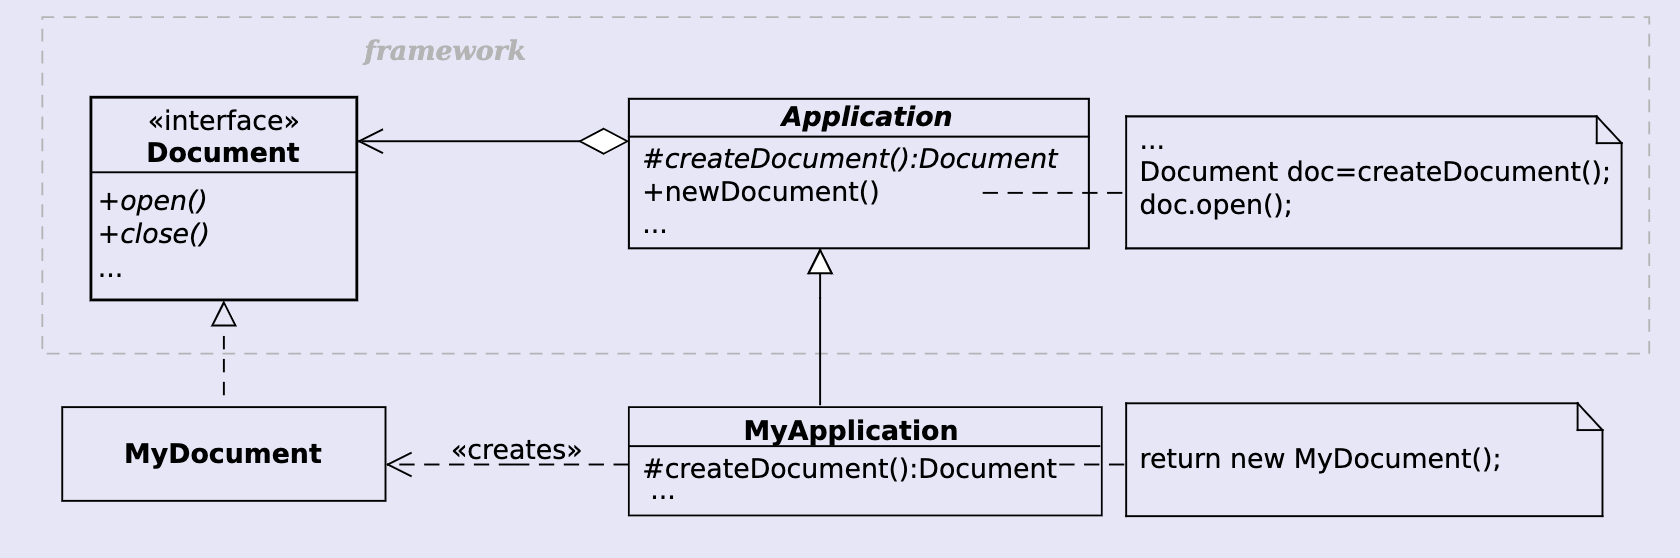
\includegraphics[width=1\linewidth]{assets/pattern/factory-method/factory-method-esempio.png}
\end{figure}

\paragraph{Soluzione} La classe Application è responsabile della gestione di oggetti conformi all’interfaccia Document e della loro creazione. Application sa solo quando dovrà creare un nuovo documento ma non di che tipo né come dovrà farlo. La responsabilità è spostata all’esterno del framework: le sottoclassi di Application devono fornire l’implementazione del metodo factory \textit{createDocument()} in modo da restituire un’istanza della classe appropriata

\paragraph{Struttura e Conseguenze} Il pattern è composto da:
\begin{itemize}
    \item \textbf{Product} (Document): definisce l'interfaccia degli oggetti creati dal metodo factory;
    \item \textbf{ConcreteProduct} (MyDocument): implementa l'interfaccia Product;
    \item \textbf{Creator} (Application): dichiara il metodo factory che restituisce un oggetto di tipo Product. Può invocare \textit{createProduct()} per creare un prodotto;
    \item \textbf{ConcreteCreator} (MyApplication): sovrascrive \textit{createProduct()} in modo da restituire una specifica istanza di ConcreteProduct;
\end{itemize}


\begin{figure}[H]
    \centering
    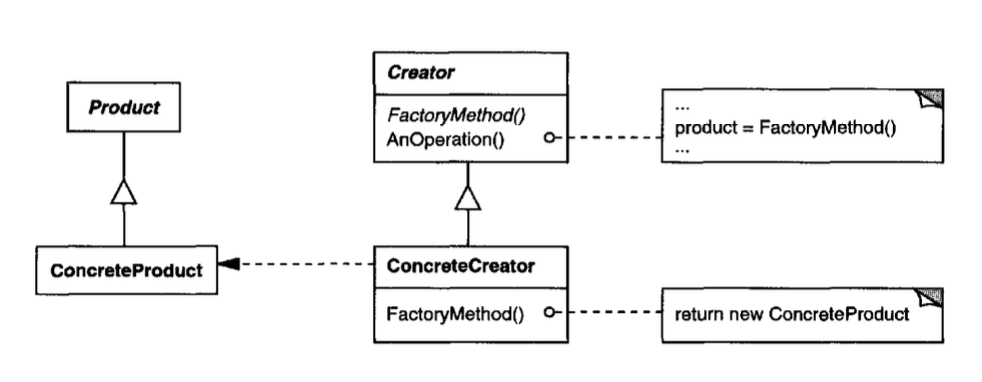
\includegraphics[width=1\linewidth]{assets/pattern/factory-method/factory-method-struttura.png}
    \caption{Class Diagram del pattern Factory Method}
\end{figure}

\begin{itemize}
    \item Elimina la necessità di riferirsi a classi dipendenti dall’applicazione all’interno del codice del framework.
    \item Gli utilizzatori potrebbero essere costretti a definire sottoclassi di Creator per creare un particolare oggetto ConcreteProduct.
    \item Fornisce un punto d’aggancio per le sottoclassi per la produzione di una versione specializzata di un prodotto.
    \item Connette gerarchie di classi parallele. Il metodo factory potrebbe invocato da oggetti diversi dal Creator.
\end{itemize}

\begin{figure}[H]
    \centering
    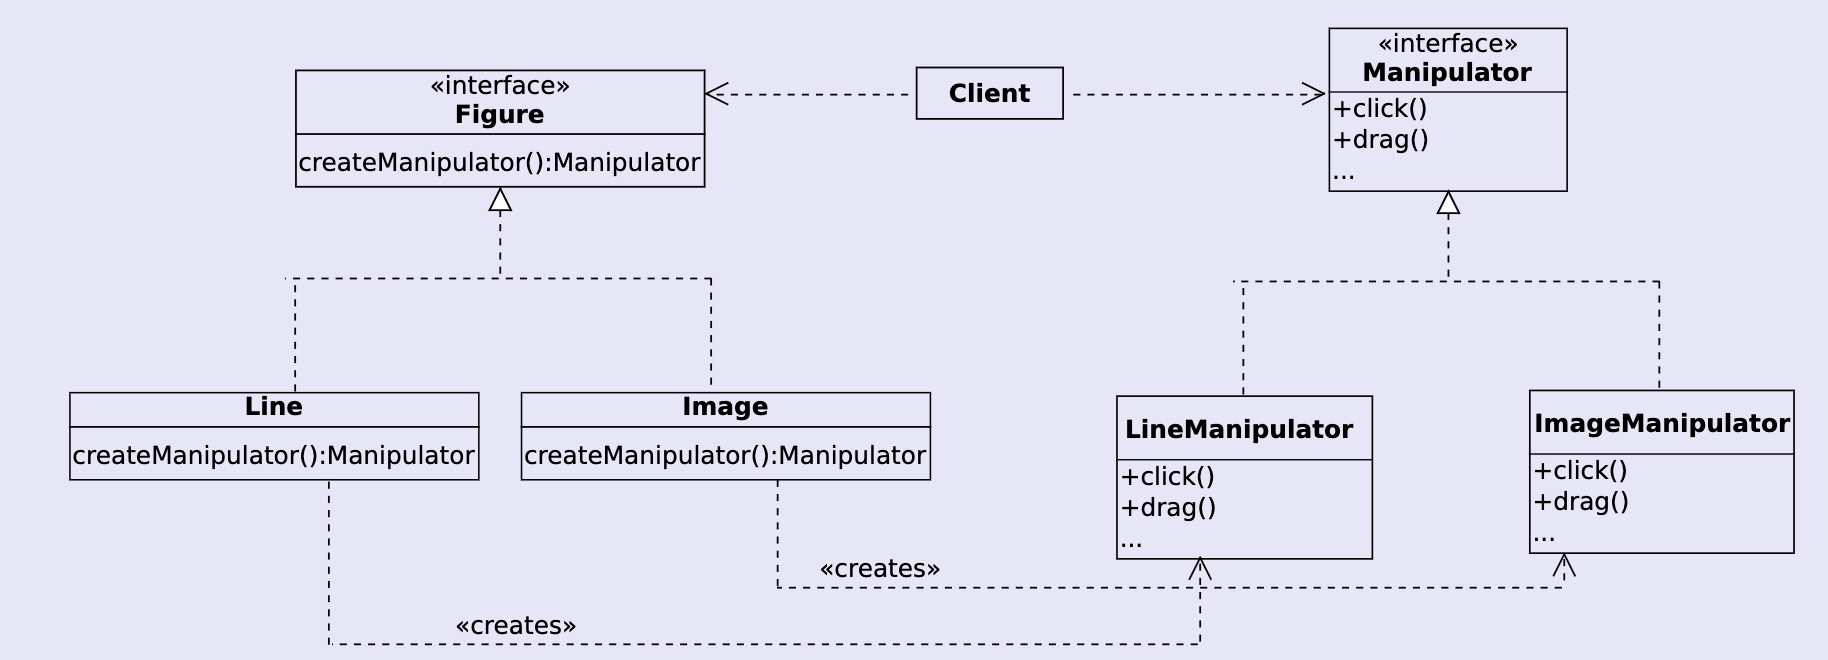
\includegraphics[width=0.8\linewidth]{assets/pattern/factory-method/factory-method-parallelo.png}
    \caption{Gerarchie di classi parallele}
\end{figure}

\begin{figure}[H]
    \centering
    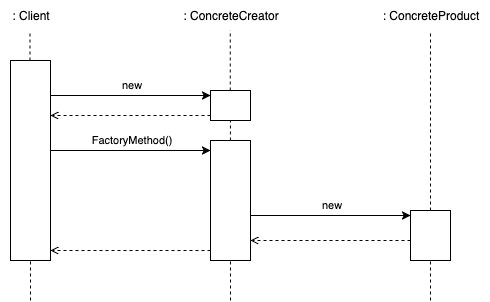
\includegraphics[width=0.8\linewidth]{assets/pattern/factory-method/factory-method-sequence.drawio.png}
    \caption{Sequence Diagram del pattern Factory Method}
\end{figure}

\newpage